\documentclass[tikz,border=5pt]{standalone}
\usepackage{fontspec}
\setmainfont{TeX Gyre Termes}
\setsansfont{TeX Gyre Heros}
\usepackage{pgfplots}
\pgfplotsset{compat=1.18}
\usetikzlibrary{patterns,positioning,arrows.meta}
\definecolor{blue}{HTML}{0072B2}
\definecolor{green}{HTML}{009E73}
\definecolor{orange}{HTML}{E69F00}
\definecolor{red}{HTML}{D55E00}
\definecolor{grey}{HTML}{8D9399}
\pgfplotsset{every axis/.append style={width=8.1cm,height=5.3cm,
font=\small,axis lines=left,axis line style={grey},tick align=outside,
enlarge x limits=.18,ymajorgrids=true,grid style={grey!18},
tick label style={font=\small},label style={font=\small},
nodes near coords style={font=\small,/pgf/number format/fixed,/pgf/number format/precision=2,/pgf/number format/1000 sep={,}},clip=false}}
\begin{document}
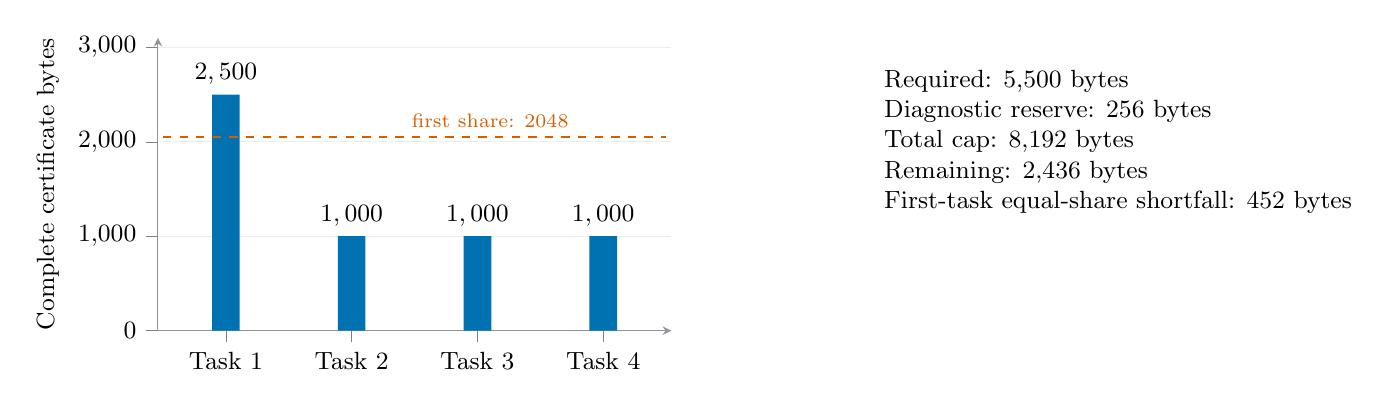
\begin{tikzpicture}
\begin{axis}[ybar,xtick={0,1,2,3},xticklabels={Task 1,Task 2,Task 3,Task 4},ymin=0,ymax=3100,ylabel={Complete certificate bytes},nodes near coords]
\addplot[fill=blue,draw=none] coordinates {(0,2500) (1,1000) (2,1000) (3,1000)};
\draw[red,dashed,thick] (axis cs:-.5,2048)--(axis cs:3.5,2048);\node[red,anchor=west,font=\scriptsize] at (axis cs:1.4,2220) {first share: 2048};
\end{axis}
\node[align=left,anchor=west,font=\small] at (9.1cm,2.4cm) {Required: 5,500 bytes\\Diagnostic reserve: 256 bytes\\Total cap: 8,192 bytes\\Remaining: 2,436 bytes\\First-task equal-share shortfall: 452 bytes};\end{tikzpicture}
\end{document}
